% IEEEAerospace2012.cls requires the following packages: times, rawfonts, oldfont, geometry
\documentclass[twocolumn,letterpaper]{IEEEAerospaceCLS}  % only supports two-column, letterpaper format

% The next line gives some packages you may find useful for your paper--these are not required though.
%\usepackage[]{graphicx,float,latexsym,amssymb,amsfonts,amsmath,amstext,times,psfig}
% NOTE: The .cls file is now compatible with amsmath!!!

\usepackage[]{graphicx}    % We use this package in this document
\usepackage{amsmath}
\usepackage{multirow}
\usepackage{hyperref}
\hypersetup{
    colorlinks=true,
    linkcolor=black,
    filecolor=black,      
    urlcolor=black,
    citecolor=black,
    draft,
}

% et al.
% \DeclareRobustCommand\onedot{\futurelet\@let@token\@onedot}
% \def\@onedot{\ifx\@let@token.\else.\null\fi\xspace}
\newcommand{\abbreviation}[1]{\emph{#1}.}
\newcommand{\etal}{\abbreviation{et~al}}

\newcommand{\ignore}[1]{}  % {} empty inside = %% comment
\newcommand\todo[1]{\textbf{\textcolor{red}{#1}}}
\graphicspath{{imgs/}}

\begin{document}
\title{Incorporating Hierarchical Information for UAV based Semantic Mapping}

\author{%
    Nicolas Mandel\\
    Queensland University of Technology\\
    Australian Centre for Robotic Vision\\
    QUT Centre for Robotics\\
    nicolasjohann.mandel@hdr.qut.edu.au
    \and
    Michael Milford\\
    Queensland University of Technology\\
    Australian Centre for Robotic Vision\\
    QUT Centre for Robotics\\
    \and
    Felipe Gonzalez\\
    Queensland University of Technology\\
    Australian Centre for Robotic Vision\\
    QUT Centre for Robotics\\
    %%%% IMPORTANT: Use the correct copyright information--IEEE, Crown, or U.S. government. %%%%%
    \thanks{\footnotesize 978-1-7281-7436-5/21/$\$31.00$ \copyright2021 IEEE}              % This creates the copyright info that is the correct 2021 data.
    %\thanks{{U.S. Government work not protected by U.S. copyright}}         % Use this copyright notice only if you are employed by the U.S. Government.
    %\thanks{{978-1-7281-7436-5/21/$\$31.00$ \copyright2021 Crown}}          % Use this copyright notice only if you are employed by a crown government (e.g., Canada, UK, Australia).
    %\thanks{{978-1-7281-7436-5/21/$\$31.00$ \copyright2021 European Union}}    % Use this copyright notice is you are employed by the European Union.
}



\maketitle

\thispagestyle{plain}
\pagestyle{plain}



\maketitle

\thispagestyle{plain}
\pagestyle{plain}

\begin{abstract}
Power, size and weight are major constraining factors for UAVs, which have caused researchers to investigate alternative information representations, such as semantics, to reduce the computational load onboard UAVs. However, the connection between spatial and semantic information has not been fully explored and the literature on including semantic information for UAV navigation is limited. This paper provides a new taxonomoy on spatial and semantic relations through consideration of a selected subset of the literature. Concepts of semantic information are related with spatial maps and two hypotheses for improving algorithms based on the literature are generated. The algorithms are tested in numerical simulations on the task of semantic mapping and the effects of influential parameters are examined. Results indicate that a defined hierarchical structure of semantic information enables improved map reproduction. The proposed algorithm exhibits the potential to improve the use of semantic information in UAV deployment scenarios, such as agriculture, search and rescue and industrial inspections.
\end{abstract}


\tableofcontents

%%%%%%%%%%%%%%%%%%%%%%%%%%%%%%%%%%%%%%
\section{Introduction} \label{sec:Intro}
%%%%%%%%%%%%%%%%%%%%%%%%%%%%%%%%%%%%%%
Limitations in power, size and weight in UAVs have resulted in researchers exploring alternative approaches of representing information to reduce the computational load onboard UAVs. Contextual information is often used for navigation, with semantics at the frontier of contemporary robotics research showing promising results. Kostavelis and Gasteratos define semantics as ''[...] related to the study between signs and the things to which they refer, that is their meaning.''~\cite{kostavelis_semantic_2015}. Semantic information has been included into the passive part of SLAM~\cite{cadena_past_2016,zhang_hierarchical_2019}, as well as into active path planning~\cite{koch_automatic_2019,alirezaie_exploiting_2017}.  However, in terms of semantic signal source, multiple levels of signals are possible, such as individual objects, regions or areas~\cite{kostavelis_semantic_2015}. These cause new problems for definining successful navigation, as highlighted by Anderson~\etal~\cite{anderson_evaluation_2018}. Furthermore, recent advances in Computer Vision have produced a wide range of different sensors signals to be annotated with semantic information, such as pixel-level segmentation, object detection or scene classification~\cite{alom_history_2018}, which operate on different spatial levels.
\begin{figure}[t]
    \centering
    \includegraphics[width=3.25in]{Aerial15.png}\\
    \caption{\bf{An example of a UAV performing a semantic mapping task on an urban area, demonstrated by assigning colors to grid maps. Blue fields represent cars, green fields houses, gray fields roads. Light green denotes grass and dark green trees. The black dashed square represents the field of view of the UAV.}}
    \label{fig:AerialImg}
\end{figure}
The influence of these sensor signals on the level of names on conventional robotics algorithms, such as filters and path planners, is an active field of research~\cite{kostavelis_semantic_2015,cadena_past_2016,anderson_evaluation_2018}. UAVs are impacted by unique viewing angles, as well as risk-averse requirements and hard constraints on computational resources~\cite{mandel_method_2020,gonzalez_unmanned_2016,boroujerdian_mavbench_2018}, which add additional complexity to the problem of semantic based navigation. Figure~\ref{fig:AerialImg} illustrates the context where the UAV has a field of view and semantic classes are estimated from a top-down view and assigned to a map of grid cells. The classes for this example are house, vehicle, grass, road and tree.  

Two key contributions are presented, the first of which leads to the second. Firstly, a review of a selected subset of the literature in this area is conducted to create a taxonomy that enables the key factors in successful utilization of semantic information. Using these new insights, algorithms are proposed and evaluated in functionally-relevant numerical simulations according to a generic autonomous algorithm development framework~\cite{ladosz_generic_2019}. Initial results demonstrate the potential of the approach to improve semantic mapping performance.

This paper is split into two parts: the first part is concerned with a taxonomy of a selected subset of literature on semantic navigation. The second part contains the proposal of algorithms based on conclusions drawn from the literature, which are evaluated in numerical simulations. Each of these sections contain their own structure of Methodology, Results and Discussion, with a final Conclusion section summarizing the results and providing an outlook.  This research is directed towards enhancing the performance of a module which is tasked with extracting and evaluating the semantic information during UAV path planning in a navigational framework~\cite{mandel_towards_2020}.

\section{Literature Taxonomy} \label{sec:Lit}
In this paper we evaluate a selected subset of literature, which combines semantic signals with spatial information in robotics to demonstrate the state of the research. The literature is categorised with respect to different dimensions.
\subsection{Methodology} \label{ssec:LitMet}
Twenty-six papers were selected for this research. The papers are sorted according to the following three dimensions and the methods employed in those papers are extracted:
\begin{enumerate}
    \item Robot Type
    \item Spatial Map
    \item Semantic Map
\end{enumerate}
Significant research is briefly summarized along with the rough timeframes of the projects to contextualize the progress in the field. The main contributions are extracted and the form of inclusion of semantic information with spatial information is highlighted.

\begin{figure}[t]
    \centering
    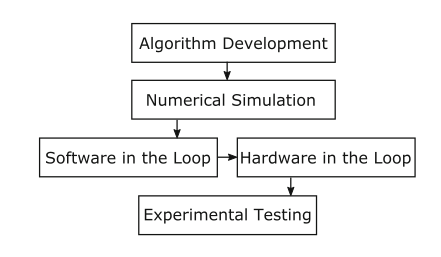
\includegraphics[width=3.25in]{2-3DevelopmentCycle.png}\\
    \caption{\bf{A generic autonomy development cycle as proposed by Ladosz~\etal~\protect\cite{ladosz_generic_2019}}}
    \label{fig:DevProcess}
\end{figure}

\subsection{Results} \label{ssec:LitRes}
The taxonomy of the selected literature illustrates the methods employed in the literature with respect to the spatial, semantic and robot type-dimensions.

\begin{figure*}
    \centering
    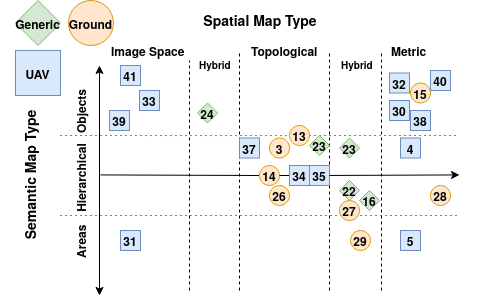
\includegraphics[width=\textwidth]{Lit-14.png}
    \caption{\bf{
        Categorization of the included literature. The y-axis represents the level of the semantic information, whether objects, areas or a hierarchical combination were used. The x-axis represents the spatial information, ranging from image space over topological associations to metric space. The colors represent the type of robot used in the research, with blue denoting UAVs, orange denoting ground robots and green generic research.
    }}
    \label{fig:LitRes}
\end{figure*}
Figure~\ref{fig:LitRes} shows the results of generating a taxonomic representation of the included literature. The literature extends to a selection from 1995 to 2020 and has been classified according to the spatial and semantic maps that were used, as well as the robot type employed in the research. It should be noted that in most cases image space was used to extract semantic information, however, the map retainment is considered as the defining factor for the spatial map. The majority  of research considered in this work is employing a hybrid approach on either the semantic level or the spatial level. A smaller portion considers non-hybrid information and is placed in the corners of the figure.  
\subsubsection{Generic Research} \label{sssec:LitResHis}
Five research efforts considered as ''generic'' from as early as 1995  have been included in the taxonomy of this paper.

Chown and colleagues for example~\cite{chown_prototypes_1995} researched the "what" and "where" subsystems of the human cognition and their learning over time. They captured the influence of landmark recognition, recreation of consistent Euclidean maps, as well as the importance of gateways, representing transitions between regions. Suenderhauf~\etal~\cite{sunderhauf_meaningful_2017} associated point-clouds in SLAM with labels propagated through a modern neural network. Yang~\etal~\cite{yang_visual_2018} used scene priors derived from vector representations of class names to enhance a reinforcement learning module which relies on visual cues in indoor environments. Crespo~\etal~\cite{crespo_reasoning_2018} generalised the implementation of a knowledgebase-system developed by Tenorth~\etal~\cite{tenorth_knowrob-map_2010} to a database implementation and improved the speed significantly. In 2018, Wu~\etal~\cite{wu_learning_2018} used reinforcement learning to train an agent to recognise a room and infer whether one room type is directly or indirectly accessible from another room using a Bernoulli distribution.
\subsubsection{Ground Robots} \label{sssec:LitResGro}
Eight research efforts from a timespan between 2000 and 2020 have been considered in this taxonomy. Contemporary image processing techniques have accelerated semantic spatial research through significant improvements in reliability and robustness of classification and localisation in image space~\cite{alom_history_2018}.

Kuipers~\cite{kuipers_spatial_2000} connected places, defined as 0D ''points'', through 1D ''paths'' with 2D ''regions'' in topological maps. The proposed maps had a sensory and control level, a causal level, a topological level and a metrical level, all of which were connnected hierarchically. Together with his colleagues, Kuipers~\cite{kuipers_local_2004} also conducted experiments where local metric room representations were linked through topological constraints. Galindo~\etal~\cite{galindo_robot_2008} connected a spatial hierarchical representation consisting of areas and objects with a terminological box and connected between these two in a deterministic manner to enable inference and path planning. Borkowski~\etal~\cite{borkowski_towards_2010} assigned a hierarchical place taxomony based on house representations from architecture to a metric map and performed path-planning within this map while considering semantic constraints. Tenorth~\cite{tenorth_knowrob-map_2010} built a topological representation of abstract objects and locations and associates these in a hierarchical fashion to enhance task planning by incorporating the relations of objects. Krishnan and Krishna~\cite{krishnan_visual_2010} constructed a hierarchical semantical-topological and explored the semantic nodes before proceeding to the next. Zhang~\etal~\cite{zhang_hierarchical_2019} used a hierarchical topic model to improve the performance of a SLAM system by actively integrating the object association problem into a hierarchical dirichlet process.

Chaplot~\etal~\cite{chaplot_object_2020} won the 2020 CVPR challenge to navigate to an object goal by learning a semantic-metric map from visual cues and training a policy to generate frontier-based goals. Their research also highlighted that other RL policies were outperformed by frontier-based methods and were unable to generalize to the real-world.

\subsubsection{UAVs} \label{sssec:LitResUAV}
Thirteen UAV-based research efforts from $2013$ onwards have been included in this taxonomy, which present a variety of approaches of including semantic information. A substantial amount of literature is concerned with passive acquisition of semantic information:

Le Saux and Sanfourche~\cite{saux_rapid_2013}, Sheppard and Rahnemoonfar~\cite{sheppard_real-time_2017}, Christie~\etal~\cite{christie_semantics_2016} and Kyrkou~\etal~\cite{kyrkou_dronet:_2018}, classified top-down images taken from a UAV. Cavaliere~\etal~\cite{cavaliere_towards_2016,cavaliere_towards_2018} associated ''tracks'' coming from images with ''places'' from geospatial information to describe relations between them in a relational manner, as detailed in~\cite{landsiedel_review_2017}. The individual items were structured hierarchically to distinguish between different type of tracks, such as vehicles and humans on the first level and cars, motorcycles and trucks on the second level. Drouilly~\etal~\cite{drouilly_semantic_2015} developed a metric to evaluate the semantic quality of a path through an environment depending on the distribution of objects and the observation quality.

Semantic information has also been employed in active navigation. Maturana~\etal~\cite{maturana_looking_2017} annotated a 2.5D map with detection of cars and developed a system to approach the cars using UAVs. Maravall~\etal~\cite{maravall_navigation_2017} used the image entropy to navigate through a topological map to semantically salient places. Alirezaie~\cite{alirezaie_exploiting_2017} developed a RRT implementation that discards semantically inadmissible points through geospatial information associated with the waypoints and significantly improved planning time for longer distances. Dang~\etal~\cite{dang_autonomous_2018} employed an object detector on top of a voxel grid to detect humans and bicycles. Koch~\etal~\cite{koch_automatic_2019} respected semantic constraints during the path planning step for 3D reconstruction using UAVs while maintaining the quality of the reconstruction.
Toudeshki~\etal~\cite{toudeshki_robust_2018} combined a visual teach-and-repeat approach with an object detector to funnel the UAV to follow a path.
\subsubsection{Summary} \label{sssec:ResLitSum}
Fusing semantic information with spatial information for navigation, mapping or task-planning has been an active field of research for the past decades. A majority of research fuses information into hybrid models, either on the semantic or on the spatial axis. This is demonstrated by the centralised cluster as shown in figure~\ref{fig:LitRes}. UAV research is more spread out than other approaches in this figure.

The centralised clustering indicates that research has benefitted from hybrid approaches, which have not yet been translated to UAVs due to the hurdle of additional complexity. A significant portion of the included literature incorporated a hierarchical structure, most commonly in the form of an associative connection between ''areas'' -- or ''rooms'' -- and ''objects''~\cite{galindo_robot_2008,zhang_hierarchical_2019,chaplot_object_2020,tenorth_knowrob-map_2010,borkowski_towards_2010,kuipers_spatial_2000,cavaliere_empowering_2018,cavaliere_towards_2016}. Based on these insights a hybrid algorithm, which is to be tested in a simulation scenario with reduced complexity, is proposed.

\section{Simulations} \label{sec:Sim}
\begin{figure*}[t]
    \centering
    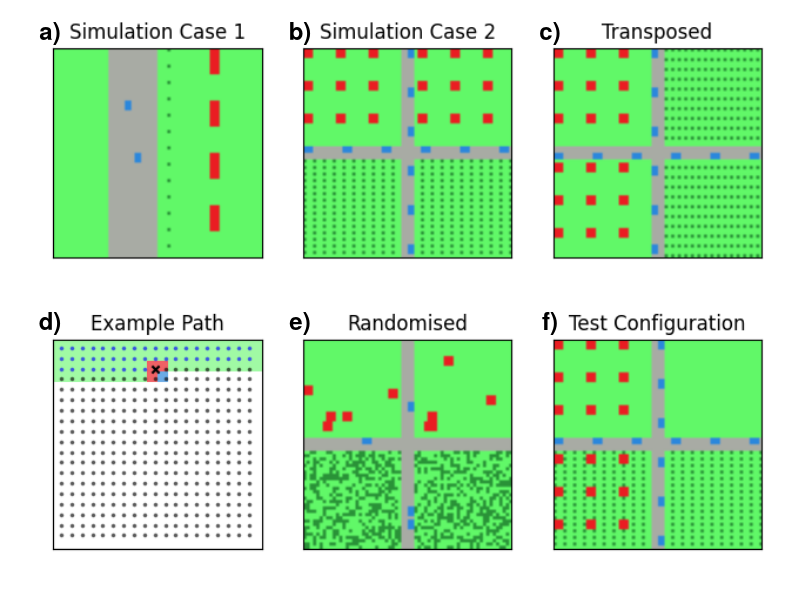
\includegraphics[width=0.8\textwidth,height=3.5in]{SimComp13.png}
    \caption{\bf{
        Examples of the simulations abstracted from possible aerial images, see figure~\ref{fig:AerialImg}. Colors are intended to represent different semantic classes according to table~\ref{tab:colors}, see figure~\ref{fig:AerialImg} for context. a) shows the first simulation environment $s=1$, b) the second environment $s=2$. c) a transposed configuration, $t=1$, e) randomised configuration $r=1$ and f) a test configuration $c=1$ as defined in table~\ref{tab:params}. d) shows an example path, with the $\times$ representing the UAV, the green cells the previously seen cells, the red cells the currently seen and already known cells and the blue cells the cells predicted at $t_{-1}$ 
    }}
    \label{fig:SimCase}
\end{figure*}
The literature taxonomy uncovered that a substantial part of semantics research in robotics benefits from hybrid approaches along the spatial and semantic axes, denoted by the centralised cluster in figure~\ref{fig:LitRes}. UAVs are constrained by additional layers of complexity in translation of conventional semantic detection methods and deployment~\cite{mandel_method_2020}. As a result, the development pipeline shown in figure~\ref{fig:DevProcess} is followed to evaluate the proposed approach in numerical simulations. Based on observations from the literature, an algorithm is proposed that uses information in a hierarchical manner, such as the commonly used association between ''areas'' and ''objects''~\cite{tenorth_knowrob-map_2010,galindo_robot_2008,chaplot_object_2020,wu_learning_2018}.

\subsection{Methodology} \label{ssec:SimMet}
Numerical simulations are conducted to expose influences of parameters of the mapping pipeline and differences between algorithms. Figure~\ref{fig:SimCase} shows the setup of the simulation. The task is to recreate a map from sequential, noisy semantic observations. The map is an evenly spaced 2D grid $M \times M$ defined by a one-hot vector of the true identity, $x_{i,j} = \{0,..., 1, ..., 0\}_K$, with $K$ indicating the number of classes. The probability of making an observation $z$ is given by $p(z\mid x)$. The pose is assumed to be known for the entire trajectory. At each time increment $t$ the UAV observes cells within its field of view $f$, receives a one-hot observation proportional to $p(z\mid x)$ and updates the posterior of each map cell given by Bayes' rule as:
\begin{equation} \label{eq:Bayes}
    p(x\mid z) = \frac{p(z\mid x) p(x)}{p(z)}
\end{equation}
which is equivalent to the performance of any given detector~\cite{alom_history_2018}.

The UAV is following a conventional lawnmower pattern, where the stride in both dimensions is defined through a desired overlap $o$ and field of view $f$~\cite{shetty_implementation_2020}. Figure~\ref{fig:SimCase} d) shows a snapshot of the simulation at time $t=47$. The green cells in the figure indicate the cells that have already been observed, the red cells the current $f$ of the UAV, which is marked by the black $\pmb{\times}$. The blue cells denote the cells where the prior $p(x)$ has been predicted at $t_{-1}$, based on the posterior of the red cells.

Four algorithms are compared in parallel with the same sampled observations. In all cases, only the prior $p(x)$ for each cell is predicted and all subsequent observations are incorporated according to equation~\ref{eq:Bayes}. In the baseline case (algorithm 1), the prior for each cell $p(x)$ is uniform over all classes $K$, which is denoted as a Naive Bayes Filter. In the other three cases, spatial correlation is incorporated into the prior. The prediction for the cells is made by extracting the next waypoint $t_{+1}$ and evaluating all cells that will be visible within the field-of-view $f$ at that timestep. In the second algorithm (algorithm 2), yet unobserved cells receive a prior which is a linear combination of the uniform prior and the posterior of the already observed cells. The posterior probability is weighted by a mixing parameter $\alpha \in [0, 1]$, as well as the ratio of number of observed cells divided by total cells -- defined through the overlap $o$ and $f$ -- and used as a prior for the yet unobseved cells.

The other two algorithms are based on assumptions drawn from the results of the literature taxonomy as detailed in section~\ref{ssec:LitRes}. Incorporating information in a hierarchical context has proven successful in related semantic fields, such as speech processing~\cite{fine_hierarchical_1998} and topic modelling~\cite{blei_latent_2003}. These approaches have been succesfully adapted to related domains, such as image annotation~\cite{fei-fei_bayesian_2005,lienou_semantic_2010} or SLAM~\cite{zhang_hierarchical_2019}. Some algorithms have incorporated the hierarchical semantic information succesfully for the purpose of navigation~\cite{koch_automatic_2019,chaplot_object_2020,wu_learning_2018,alirezaie_exploiting_2017}.

Two algorithms  that recalculate the prior based on hierarchical information are proposed: the prior is calculated according to an assumed distribution of ''areas'' -- $u$ -- groupings of cells. These groupings require the definition of $p(x\mid u)$ -- the distribution of ''objects'' in a given ''area'' -- and $p(u)$, as well as the number of groupings, which is usually smaller than $K$, analogous to topic modelling~\cite{blei_latent_2003}. In the third algorithm (algorithm 3), every map cell is assigned a fixed prior of $p(x_{t=0}) = p(x\mid u) p(u)$. In the fourth algorithm (algorithm 4) $p(u)$ is updated dynamically by using the observations of each cell within $f$, with a fixed $p(x\mid u)$, which leads to a new dynamically assigned $p(x)$.

Three variations of $p(u)$ and $p(x\mid u)$ -- denoted by the parameter \emph{Ptu} -- are considered. The first is a manual version, where the mixture of ''objects'' in ''areas'' $p(x\mid u)$ is estimated by the user and the distribution of ''areas'' $p(u)$ in the map as well. In the second and third version, $p(x\mid u)$ and $p(u)$ are derived through Monte-Carlo simulations described in section~\ref{ssec:SimMetMC}. $K=5$ and $3$ are used for the simulations, because the small number allows for interpretability, visual simplicity and numerical stability when defining and evaluating simulation cases.

Robotics research is often constrained by the overlap of classes available in detection and simulation environments~\cite{chaplot_object_2020}, such that $5$ is a reasonable approximation for numerical research. The chosen classes are distributed according to different scales, with one class being dominant in the map, occupying over $70$~\% of the cells in the majority of cases, while another class occupies less that $1$~\%. Furthermore, the classes occupy different connected regions of the map, ranging from $1$ isolated cell to multiples of the field-of-view, which allows the investigation how different scales influence the performance.

The simulation cases can be transposed -- indicated by $t$ in figure~\ref{fig:SimCase} c)-- to evaluate the influence of the path planning direction on the predictive performance. The second simulation environment has further boolean parameters, that randomize the placement of objects in quadrants $r$, as well as a parameter that mixes two quadrants $c$ to illustrate visual diversity and reduce uniformity of areas.

The simulation cases are displayed in figure~\ref{fig:SimCase} and table~\ref{tab:params} shows the parameters that have been varied.
\begin{table}[]
    \renewcommand{\arraystretch}{1.3}
    \caption{\bf Color indicators}
    \label{tab:colors}
    \centering
    \begin{tabular}{|r||l|}
        \hline
        \bfseries Color      & \bfseries Class Name    \\
        \hline \hline
        Red &  House\\
        \hline
        Gray  & Road         \\
        \hline
        Light Green     & Grass              \\
        \hline
        Dark Green & Tree           \\
        \hline
        Blue & Vehicle \\
        \hline
    \end{tabular}
\end{table}
\begin{table}[]
    \renewcommand{\arraystretch}{1.3}
    \caption{\bf Parameter variations for the simulations}
    \label{tab:params}
    \centering
    \begin{tabular}{|r||c|l|}
        \hline
        \bfseries Name      & \bfseries Symbol & \bfseries Values       \\
        \hline \hline
        Map Dimensions & $M$ & $48, 64$\\
        \hline
        Field of View  & $f$              & $1, 2$ \\
        \hline
        Overlap     & $o$              & $0.25, 0.5, 0.75$         \\
        \hline
        Accuracy & $p(z\mid x)$              & $0.6, 0.7, 0.8, 0.9, 0.95$        \\
        \hline
        Prior $p(x\mid u)$ & $ptu$ & $0, 1, 2$ \\
        \hline
        Environment & $s$ & $1, 2$ \\
        \hline
        Random & $r$ & $0, 1$ \\
        \hline
        Transpose & $t$ & $0, 1$  \\
        \hline
        Test & $c$ & $0, 1$  \\
        \hline
    \end{tabular}
\end{table}
The mixing parameter $\alpha$ is evaluated in a preliminary set of experiments, where $\alpha \in [0, 0.2, ..., 1]$ and therefore not included in table~\ref{tab:params}.

Figure~\ref{fig:SimCase} illustrates the basic variations for the simulation environments. ~\ref{fig:SimCase} a) is the first environment $s=1$, which is also used for the Monte-Carlo simulations -- detailed below --  and excluded from the evaluation. ~\ref{fig:SimCase} b) shows the second environment $s=2$, and~\ref{fig:SimCase} c) a transposed environment $t=1$.~\ref{fig:SimCase} e) shows a case where the placement of objects within their quadrants is randomised $r=1$.~\ref{fig:SimCase} f) shows a test environment $c=1$ with partial tranpose, which convolutes the definition of an ''area'' as a section identifiable by its composition of ''objects''. The colours are indicators of types of classes and can be interpreted as shown in table~\ref{tab:colors}, however, are not limited to the named classes.~\ref{fig:SimCase} d) shows an example path, with the green colour indicating the already observed fields, red the already seen fields at $t_{-1}$ and blue the previously unseen fields, which are predicted. All combinations are used for the simulations.
\subsubsection{Monte-Carlo simulations} \label{ssec:SimMetMC}
\begin{figure*}[t]
    \centering
    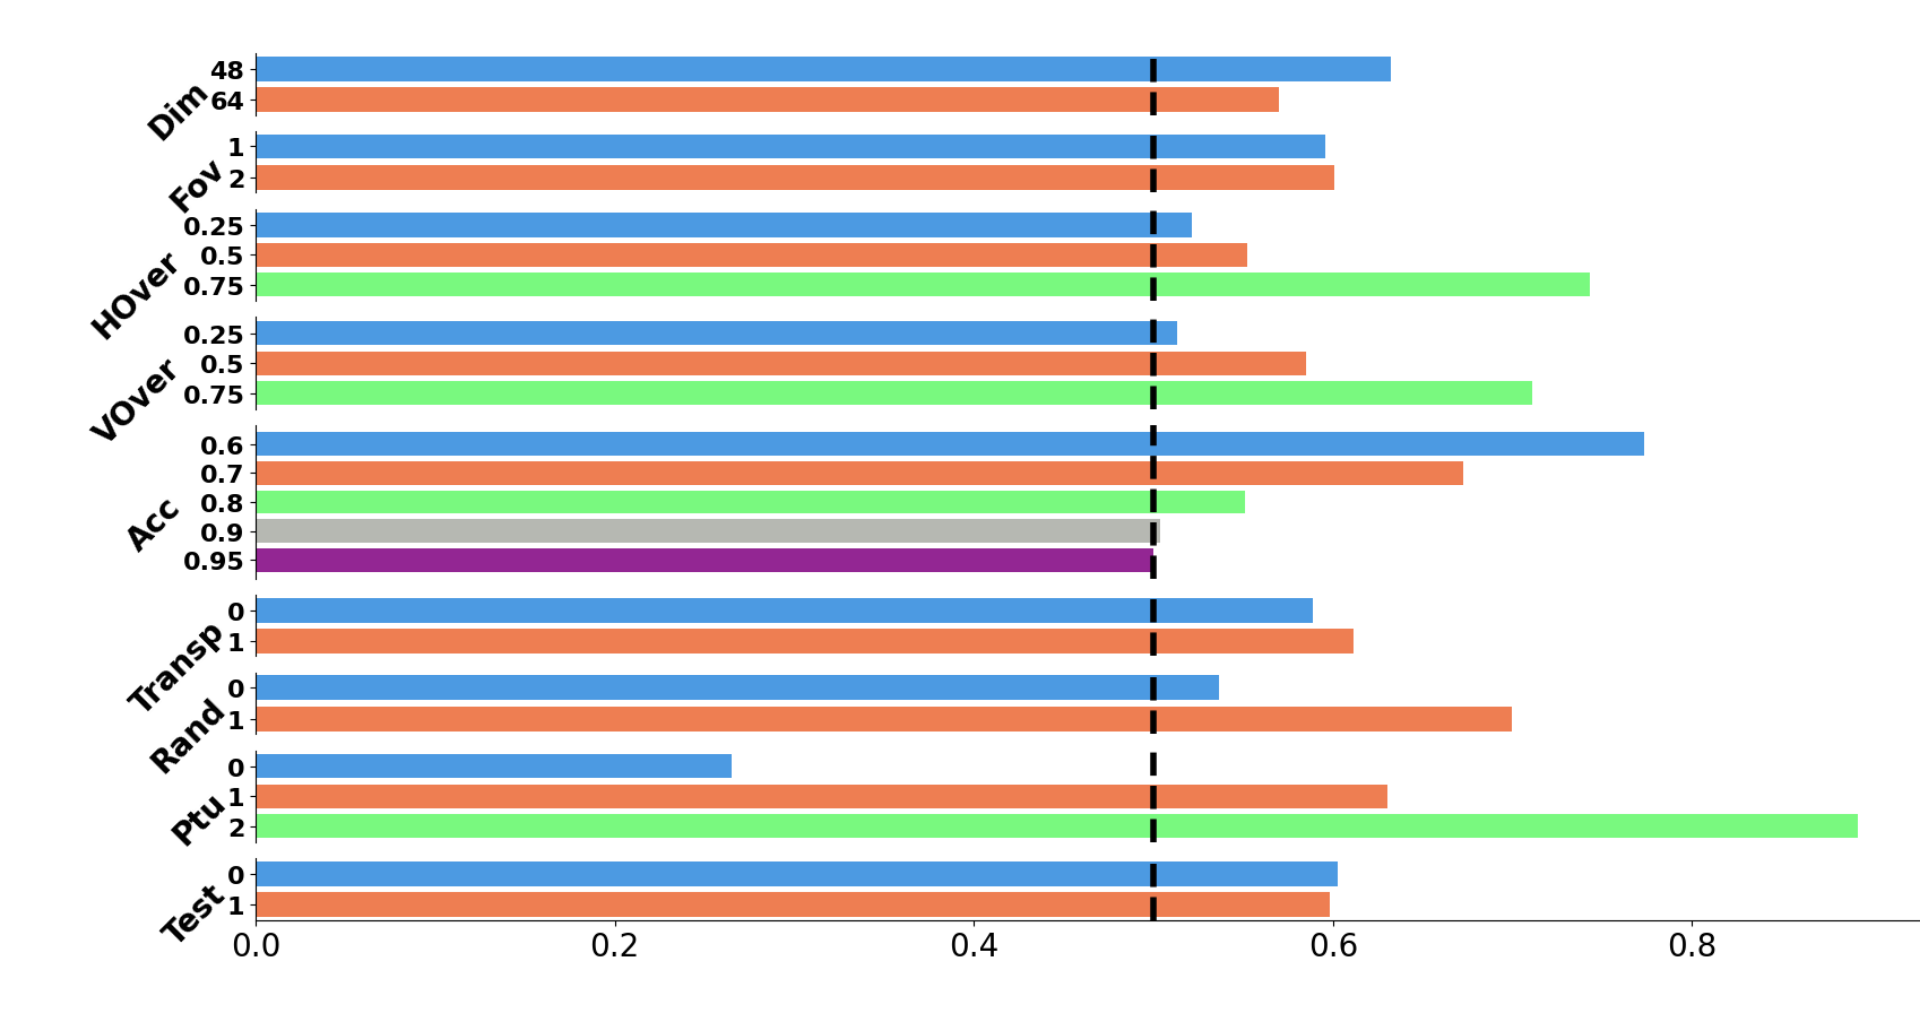
\includegraphics[width=\textwidth]{Results-15.png}
    \caption{\bf{
        Relative results related through equation~\ref{eq:eval} of the two best performing algorithms, Algorithm 2 and the Proposed Algorithm 4. The entropies calculated by equation~\ref{eq:Entropy} were subtracted from one another and related through equation~\ref{eq:eval}. The vertical black dashed line indicates the $\mathbf{50}$\% threshold. Values lower than the threshold represent a worse performance of the proposed algorithm 4. Colors serve to indicate differences in parameters. 
    }}
    \label{fig:Res}
\end{figure*}
$1000$ simulations with fixed $o=0.5$, $f=2$ and
\begin{equation} \nonumber
    p(z\mid x)=
    \begin{cases}
        0.8,~\text{for}~k=x \\
        \frac{1-0.8}{K-1},~\text{otherwise}
    \end{cases}
\end{equation}
are run on the first environment. $p(u)$ and $p(x\mid u)$ are sampled from a simplex and the performance of each algorithm as defined in section~\ref{ssec:SimMetEval} and $p(u)$ and $p(x\mid u)$ are saved if:
\begin{enumerate}
    \item The log-likelihood is smaller than the current smallest
    \item The difference between the predicted algorithm and the dynamic algorithm is bigger than the current biggest
\end{enumerate}
The final best results are used as parameters $p(u)$ and $p(x\mid u)$ for additional simulations as defined in section~\ref{ssec:SimMet}.
\subsubsection{Evaluation}\label{ssec:SimMetEval}
The reproduction quality of the posterior map for each individual state was evaluated with the sum over the log-likelihoods for each cell $m_{i,j}$, defined by:
\begin{equation} \label{eq:Entropy}
    H = - \sum_{i,j,k} p_{i,j,k}~ln(q_{i,j,k})
\end{equation}
is calculated, where $p$ represents the true state and $q$ the estimated map state.

For the comparison of different algorithms running with the same parameters, the log-likelihoods for each individual case are subtracted from another and the count of the positive and negative samples indicate the relative quality of the reproduction:
\begin{equation} \label{eq:eval}
    \frac{pos}{pos+neg} \in [0, 1]
\end{equation} If the value is below $50$\%, the algorithm performs worse than its compared baseline. This metric is chosen as a robust indicator, which is not affected by large variances for each simulation run caused by the different parameters. 
Only the second simulation environment is included in the evaluation, since the first simulation environment was used in the Monte-Carlo simulationto generate sample probability vectors, as described above.

\subsection{Results} \label{ssec:SimRes}
Numerical simulations were conducted to test the performance of the algorithms under different conditions. Figure~\ref{fig:Res} displays the results of the numerical simulations evaluated on the second simulation environment, $s=2$. Preliminary experiments showed that the second algorithm, which predicts yet unobserved cells with a mixture of $\alpha = 0.5$ always outperformed the weakest baseline and largely outperformed the second, hierarchical baseline. Therefore, results are presented which compare the hierarchical dynamic prediction of $p(x)$ through $p(u)$ and $p(x\mid u)$ with the prediction through the mixture component of $\alpha = 0.5$. A total of $1975$ simulation cases are included in this evaluation. The height of the bar indicates the percentage of outperformance, as indicated by equation~\ref{eq:eval}. A value below the threshold of $50$ \% indicates a worse performance.
% go from nondescript to descript here!
The bars for \emph{Dim} and \emph{Fov} -- $f$ in table~\ref{tab:params} -- indicate that neither the dimensions of the map $M$, nor an extended field of view $f$ lead to an improvement of one algorithm over the other. \emph{Transp} and \emph{Test} -- $t$ and $c$ in table~\ref{tab:params} respectively -- also do not significantly influence the result.

The decreasing bars for the accuracy-parameter in figure~\ref{fig:Res} indicate that the influence of the prior diminishes when the detection accuracy improves, which is aligned with the intuition of Bayesian filtering, as the detections converge to the true state. The increasing performance with increasing overlap $o$ -- which is running in parallel for both axes -- show that the additional observations benefit the hierarchical algorithm more than a linear mixing. The higher value for the \emph{Rand} parameter -- $r$ in table~\ref{tab:params} -- show that even in a randomized setting, the hierarchical prediction can lead to increased performance. The low value for \emph{Ptu} case 0 shows that a manually defined detection parameter performs significantly worse, however, the high values for 1 and 2 indicate that with the right parameters for $p(u)$ and $p(x\mid u)$, the performance can increase significantly.
\begin{figure*}
    \centering
    \resizebox{\textwidth}{!}{
    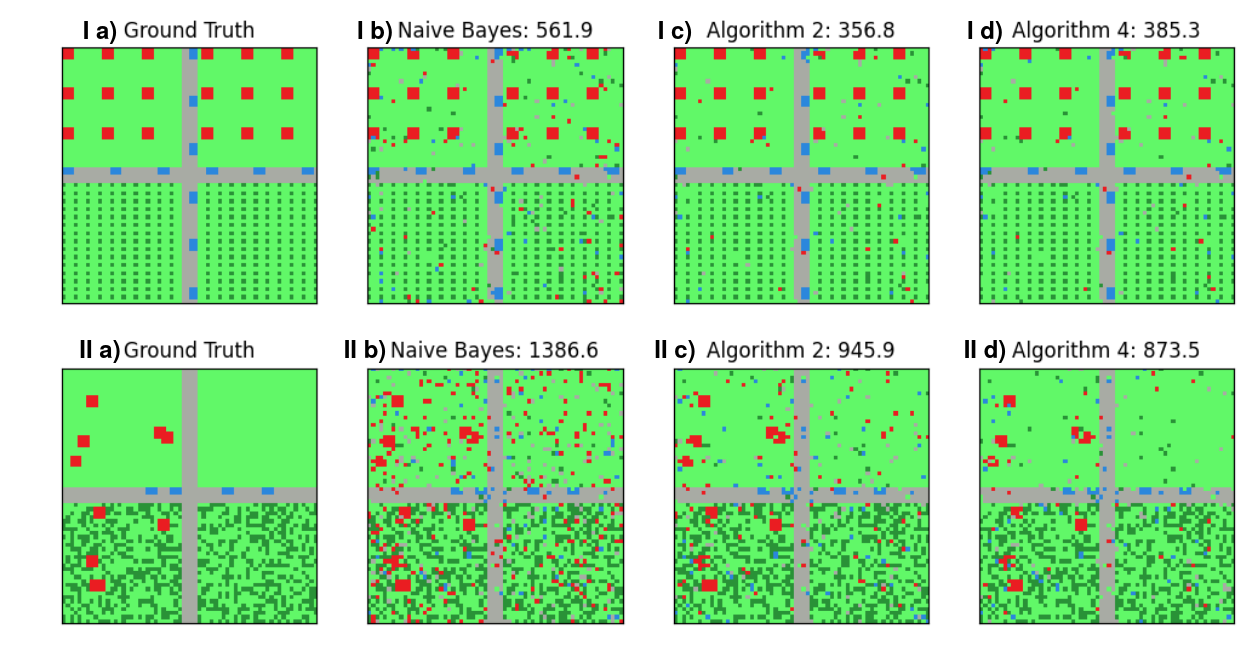
\includegraphics[width=4in]{SampRes-13.png}}
    \caption{\bf{
        Two reproduction examples for different parameters as presented in table~\ref{tab:params}. The titles indicate the algorithm, as well as the total log-liklihood as defined by equation~\ref{eq:Entropy}. Both cases show results for the second simulation environment $s=2$ with an overlap $o=0.5$, $f=1$ and $t=0$. Row I shows the results for $Ptu=0$ accuracy $0.8$ and $c=0$. Row II for $Ptu=2$,~accuracy $0.7$ and $c=1$. Columns a) show the ground truths, b) the Naive Bayes filter, c) Algorithm 2 and d) the Proposed Algorithm 4. 
    }}
    \label{fig:SampRes}
\end{figure*}

Figure~\ref{fig:SampRes} shows two reproductions of example cases, with the entropy value of the reproduction calculated by equation~\ref{eq:Entropy} in the title. Lower values indicate more accurate reproductions. Both cases show the second simulation environment used for testing, $s = 2$, with an overlap $o = 0.5$, $f = 1$ and $t= 0 $ as defined in table~\ref{tab:params}. As can be seen, both algorithms perform much better than the baseline, which is indicated by the noise in the reproduction. The first row shows an example case where the proposed algorithm was outperformed by algorithm 2, albeit by a small margin. This case represents a test configuration of $c = 0$, $r = 0$ accuracy of $0.8$ and $Ptu = 0$.  In the second row the parameters are: $c =1$, $r = 1$, accuracy $0.7$ and $Ptu = 2$.
Despite performing better than the other algorithms, the reproduction is much worse than with a higher detector accuracy which points to the significant influence of this parameter. This is shown by the large gap between row I and II for the Naive Bayes classifier, which assumes independence between individual cells and is therefore not influenced by spatial variations $c$ and $r$. However, in row II the log-likelihood decreases with a change in algorithm, despite the randomness and convolution throughout the map, which indicates that the proposed algorithm increases the performance, if the right spatial parameters can be retrieved. Manually defining these, despite best guesses, does not yield the desired result, as can be seen in column d) of figure~\ref{fig:SampRes} and underlined by the significant decrease with varying \emph{Ptu} in figure~\ref{fig:Res}.
\section{Conclusions} \label{sec:Concl}
This work has categorized twenty-six papers with respect to spatial map, semantic map and robot type for the purpose of gathering information on the benefits and challenges in image space, topological and metric representations. Subsequently, algorithms have been proposed that are to be used in the development pipeline shown in figure~\ref{fig:DevProcess}. The algorithms have been tested in numerical simulations before proceeding with further development steps.
\subsection{Literature Taxonomy} \label{ssec:ConclLit}
The taxonomy of twenty-six papers, even though not exhaustive, highlights significant factors that influence the synergy between semantic and spatial information. Not targeting robotics and therefore not included in the taxonomy is the relevant work by Harnad on symbolic systems~\cite{harnad_symbol_1990}, which discusses the association of sensory inputs with symbolic systems and intricate representations. Kostavelis and Gasteratos have completed an extensive literature review of semantic mapping for mobile robotics~\cite{kostavelis_semantic_2015} and Landsiedel~\etal~\cite{landsiedel_review_2017} have reviewed spatial relations in robotics. The taxonomy presented in this paper highlights the dimensions of semantic and spatial information with respect to the robot type and possible trends to drive the development of an algorithm.

The clustering of UAV-based semantic research in the corners of figure~\ref{fig:LitRes} indicates that mixing hierarchical information for UAVs is not an easy task. While enormous datasets and challenges along with unified metrics have driven computer vision research~\cite{alom_history_2018,corke_what_2020} and are starting to show the benefits in navigation~\cite{anderson_evaluation_2018,chaplot_object_2020}, UAVs are facing additional challenges.
On the one hand the viewpoint of UAVs compared to generalised image datasets is unique, with oblique and top-down viewing points decreasing the accuracy of detectors~\cite{richardwebster_psyphy:_2019}. On the other hand, UAVs face additional obstacles with safety considerations, as well as reduced computational capabilities~\cite{boroujerdian_mavbench_2018,mandel_method_2020}. Furthermore, increasingly complex architectures and differing quality requirements can cause difficulties in deploying algorithms~\cite{cervera_try_2019,malatova_how_2020}. 
Semantic research generally benefits from unified metrics~\cite{anderson_evaluation_2018}, simulation environments and challenges~\cite{chaplot_object_2020,yang_visual_2018}. The driving force of standardised environments and challenges~\cite{corke_what_2020} can also be seen in the UAV community, as exhibited by the development of autonomous drone racing algorithms~\cite{moon_challenges_2019}.

Chown~\etal~\cite{chown_prototypes_1995} emphasize the importance of ''gateways'' as transitions between regions, which arise naturally in manmade houses and have been used in many research efforts for ground-based vechicles~\cite{kuipers_local_2004,wu_learning_2018,krishnan_visual_2010}, however, may be difficult to define for UAVs. Where an area ends and another begins may be ambiguous for large outdoor environments, which are usually covered by UAVs~\cite{vanegas_novel_2018,shetty_implementation_2020}, whereas rooms often provide a natural separation in indoor environments. Furthermore, definitions of semantic area, region, or scene, if representing a spatial extent, could not be identified from the literature and the borders may be fluid between all of these defintions depending on the task and research field.

\subsection{Simulations} \label{ssec:ConclSim}
The results of the simulations indicate that incorporating spatial correlation can benefit the assignment of class names to grid cells, which is aligned with robotic occupancy grid mapping approaches, as well as the intuition behind convolutions and filter kernels. The inclusion of explicit hierarchical information into a mapping pipeline can be beneficial, but is largely dependant on the robustness of the model, much like topic modelling approaches~\cite{fei-fei_bayesian_2005,blei_latent_2003}.

In this research, important hardware parameters such as flying velocity and battery charge~\cite{boroujerdian_mavbench_2018} have been omitted for simplicity. Furthermore, the simulation environment is a reduced to a manually-defined version, because no standardised simulation environment for semantic mapping for UAVs could be identified and therefore exhibits a natural bias. The simplicity has been attempted to be counteracted through the consideration of parameters $c$, $t$ and $r$ to increase the diversity of test cases.   
The reliance on detection parameters is demonstrated through the significant drop in performance for \emph{Ptu} as seen in figure~\ref{fig:Res} and the convergence of the performance with increasing accuracy. With perfect detectors the filtering approach would not be necessary, however, despite increasing performance~\cite{alom_history_2018} the quality of conventional detections is decreased for UAVs due to unique viewpoints~\cite{richardwebster_psyphy:_2019} and computational constraints~\cite{krishnan_sky_2020}. The hierarchical approach proposed in this research is largely dependant on the parameters $p(u)$ and $p(x\mid u)$, as clearly indicated by figure~\ref{fig:Res}, which could be learned from data with an appropriate generative model~\cite{blei_latent_2003,lienou_semantic_2010}.
\subsection{Future Work} \label{ssec:Fut}
Learning the parameters of the hierarchical model would require a formalised definition of the generative probabilistic model. Semantics, as the study of signs and the things to which they refer~\cite{kostavelis_semantic_2015}, has profound roots in language. Computer scientists working with language have put large efforts into attempting to model spoken and written language. Spoken language has employed hierarchical models of language based on the Markov assumption to separate spoken words~\cite{fine_hierarchical_1998,murphy_dynamic_2002}, which have been translated to alternative purposes, such as motion prediction~\cite{li_layered_2015} and motion recognition~\cite{oliver_layered_2002,aarno_layered_2006}. Natural Language Processing has put significant efforts into into classifying words into topics and documents (which are considered mixtures of topics) for classification and proposition~\cite{blei_latent_2003,hofmann_unsupervised_2001}, which has been adapted for the task of scene annotation in computer vision~\cite{bosch_scene_2006,fei-fei_bayesian_2005} and on satellite images~\cite{lienou_semantic_2010}. Learning the parameters from data analogous to these models would enable the model to be extended further, such as the incorporation of location uncertainty.

Further research will focus on progressing the model through an approriate generative model and an appropriate simulation environment for semantic mapping for UAVs. Subsequent tests as defined in figure~\ref{fig:DevProcess} will enable an embedding into higher-level frameworks for semantic navigation~\cite{mandel_towards_2020,vanegas_uncertainty_2016} and finally deployment on a UAV~\cite{mandel_method_2020}.

%%%%%%%%%%%%%%%%%%%%%%%%%%%%%%%%%%%%%%%%%%%%%%%%%%%%%%%%%%%%%%%%%%%%%%%%%%%%%%%%%%%%%%%%%%%%%%%%%%%%%%
\acknowledgments
This research was conducted in the context of the Australian Research Council project number CE140100016, and supported by the QUT Centre for Robotics and ARC grant FT140101229. The authors acknowledge continued support from the Queensland University of Technology (QUT) through the Centre for Robotics. N. M. acknowledges M. Xu for his technical support during the development of this work and QUT for the financial support.

%%%%%%%%%%%%%%%%%%%%%%%%%%%%%%%%%%%%%%%%%%%%%%%%%%%%%%%%%%%%%%%%%%%%%%%%%%%%%%%%%%%%%%%%%%%%%%%%%%%%%%
\bibliographystyle{IEEEtran}
\bibliography{references}


%%%%%%%%%%%%%%%%%%%%%%%%%%%%%%%%%%%%%%%%%%%%%%%%%%%%%%%%%%%%%%%%%%%%%%%%%%%%%%%%%%%%%%%%%%%%%%%%%%%%%%
\thebiography
%% This biostyle allows you to insert your photo size 1in X 1.25in
\begin{biographywithpic}{Nicolas Mandel}{Nico_Headshot_resized.png}
    received the BSc in Sports and Technology from the Otto-von-Guericke University Magdeburg and the MSc in Biomedical Engineering Sciences from the University of Applied Sciences Technikum Vienna after writing his thesis about mechanical modelling of cardiovascular treatments at the University of Cape Town. He is currently pursuing his PhD with the Australian Centre of Excellence for Robotic Vision at Queensland University of Technology, Brisbane, focussing on employing semantics for UAV navigation.
\end{biographywithpic}

\begin{biographywithpic}{Michael Milford}{Milford_2019_resized.png}
    received the Ph.D. in Electrical Engineering and the Bachelor of Mechanical and Space Engineering from the University of Queensland (UQ), Brisbane, Australia. He is currently a Professor of Robotics, Australian Research Council Future Fellow, Chief Investigator for the Australian Centre of Excellence for Robotic Vision and Deputy Director of the QUT Centre for Robotics at Queensland University of Technology, Brisbane, Australia. His research models the neural mechanisms in the brain underlying tasks like navigation and perception to develop new technologies in challenging application domains such as all-weather, anytime positioning for autonomous vehicles.
\end{biographywithpic}

\begin{biographywithpic}{Felipe Gonzalez}{Felipe_resized.jpg}
    is an Associate Professor (UAV) in the Science and Engineering Faculty, QUT and the QUT UAV Remote Sensing Group. He holds a BEng(Mech) and a PhD from the University of Sydney. His research explores bioinspired optimization, uncertainty based UAV path planning and UAV for environmental monitoring. He currently leads two ARC Discovery Projects. His research focuses on developing UAVs with high levels of cognition to assist in understanding, exploring and protecting natural and physical environments. Felipe is a Chartered Professional Engineer and member of professional organizations including the RAeS,IEEE and AIAA
\end{biographywithpic}



\end{document}
